\documentclass[12pt,a4paper]{article}
\usepackage[utf8x]{inputenc}
\usepackage{ucs}
\usepackage[english]{babel}
%\usepackage[ngerman]{babel}
\usepackage{svg}
\usepackage{amsmath}
\usepackage{amsfonts}
\usepackage{amssymb}
\usepackage{graphicx}
\usepackage{pdfpages}
\usepackage{adjustbox}
\usepackage{float}
\usepackage[a4paper]{geometry}
\usepackage[section]{placeins}
%\usepackage{showframe}

\usepackage{hyperref}

\author{Bennet Bleßmann, Sven Korfmann}
\title{LayerBased Algorithm Specification/Documantation}

\makeindex

\begin{document}

\maketitle

\tableofcontents

%master file for generating the Specs

%order of chapters not yet final
% where to put which file and what to do and not to do
\section{Guidlines}

These are our development guidlines.

\href{https://www.ietf.org/rfc/rfc2119.txt}{RFC2119}

\begin{list}{-}{}
\item The Project will be split into modules,

all modules MUST begin with \basemodule,

all packages in a modul MUST start with the modules name.

\item All main functions not for testing MUST be in the \basemodule[.main] module.

\item All test MUST be in the \basemodule[.test] module.

\item No module SHALL depend on the module \basemodule[.test]

\item No module SHALL but \basemodule[.test] MAY depend on the module \basemodule[.main]

\item Loading Graphs from file SHOULD be done in the \basemodule[.file] module

\item The Project SHOULD be implemented using the MVC pattern.

\item Models SHOULD be in the package \basemodule[.modle].

\item Views SHOULD be in the package \basemodule[.view].

\item Controllers SHOULD be in the package \basemodule[.control].

\item The module \basemodule[.api] SHOULD contain all api related stuff. %TODO

\item Code Comments and this Specification SHALL be in English.

\item The Algorithm MUST default to be deterministic.

\item Options that make the Algorithm none deterministic MUST be advanced/hidden.

\item For Randomness a PRNG SHALL be used with a configurable or fixed seed,
on re-runs the seed MUST be restored to it's initial value.

\item Magic constants SHOULD be avoided, instead use a commented constant.
\end{list}

% why are we doing what we are doing
\include{parts/Reasoning}
% How we use the the Graph and how we perform cycle breaking
\section{Model}
The Model contains the following properties:
\begin{list}{-}{}
\item Performs choosen cycle break algorithm in another thread
\item Can return graph with Property that edges were reversed
\item The state of the Graph per "Step" will be saved

\end{list}



% How we represent the the Graph and animate the steps
\section{View}
The UI will be looking like: \\
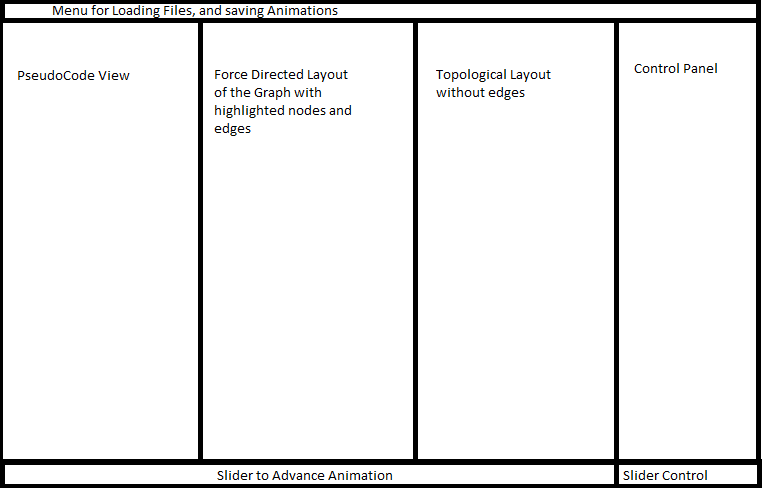
\includegraphics[width=\textwidth]{parts/UIFinished}
\begin{list}{-}{}
\item The left section will be showing the pseudocode of the current active algorithm.
\item The middle sections will show one force directed  graph on the left that will higlight Nodes the right will be ordered Topological.

\item Nodes in both graphs will be coloured dynamically.
\begin{list}{-}{}
\item Currently used node will be coloured blue in the left graph.
\item Sources will be colured cyan.
\item Sinks will be colured light gray.
\end{list}
\item Edges will be coloured as following.
\begin{list}{-}{}
\item Active edge will be coloured blue.
\item Reversed edges will be coloured green.
\end{list}
\item The right section will be a Control Panel.
\begin{list}{-}{}
\item for more information see Section Controller

\end{list}
\end{list}





% How we influence the representation
\section{Controller}
The Control panel contains:
\begin{list}{-}{}
\item A dropdown list with cycle-break algorithms
\item An option to choose verbosity
\item A slider to jump to a part of the animation
\item An option to choose how fast autoplay is
\item Buttons to play the animation forward, backward and stopping the animation
\item Buttons to step backward and and forward

\end{list}


\section{Model}
The Model contains the following properties:
\begin{list}{-}{}
\item The state of the Graph per "Step" will be saved

\end{list}






\section{Classes}


% which options do we have and what do they do
\section{Options}


% This needs to be done
\section{Minimal Viable Product}

\begin{list}{-}{}
\item A Cycle Break algorithm (Greedy)
\item Load a graph from a file (In your own input format)
\item Present a drawing of the graph
\item Be able to configure the verbosity of the animation (step forwards or backwards, run continuously, speed, level of detail, ...)
\item Be well-structured, i.e. in terms of separation of concerns (drawing, layout calculation, ...)
\item implement your visualization application in Java Swing

\item use the ElkGraph as the input format for your visualization.


\item comment the code
\end{list} % Minimum Viable Product
% If we have time we can do this
\include{parts/NTH} % Nice To Have
% We won't do this unless we have copiouse amounts of spare time (e.g. Ports)
\include{parts/OOS} % Out of Scope

\end{document}